\documentclass[12pt]{article}
\usepackage[margin=2.5cm]{geometry}
\usepackage{enumerate}
\usepackage{amsfonts}
\usepackage{amsmath}
\usepackage{fancyhdr}
\usepackage{amsmath}
\usepackage{amssymb}
\usepackage{amsthm}
\usepackage{mdframed}
\usepackage{graphicx}
\usepackage{subcaption}
\usepackage{adjustbox}
\usepackage{listings}
\usepackage{xcolor}
\usepackage{courier}
\usepackage[utf]{kotex}
\usepackage{hyperref}

\definecolor{codegreen}{rgb}{0,0.6,0}
\definecolor{codegray}{rgb}{0.5,0.5,0.5}
\definecolor{codepurple}{rgb}{0.58,0,0.82}
\definecolor{backcolour}{rgb}{0.95,0.95,0.92}

\lstdefinestyle{mystyle}{
    backgroundcolor=\color{backcolour},
    commentstyle=\color{codegreen},
    keywordstyle=\color{magenta},
    numberstyle=\tiny\color{codegray},
    stringstyle=\color{codepurple},
    basicstyle=\ttfamily\footnotesize,
    breakatwhitespace=false,
    breaklines=true,
    captionpos=b,
    keepspaces=true,
    numbers=left,
    numbersep=5pt,
    showspaces=false,
    showstringspaces=false,
    showtabs=false,
    tabsize=1
}

\lstset{style=mystyle}

\pagestyle{fancy}
\renewcommand{\headrulewidth}{0.4pt}
\lhead{CSC 369}
\rhead{Midterm 1 Solution}

\begin{document}
\title{CSC 369 Midterm 1 Solution}

\bigskip

\begin{enumerate}[1.]
    \item

    \begin{enumerate}[a)]
        \item Trap instruction is run in user mode, and privileged operation is
        run in kernel mode
        \bigskip

        \underline{\textbf{Notes}}

        \begin{itemize}
            \item \textbf{Previliged Instructions}

            \begin{itemize}
                \item Is the instruction that can run only in \textbf{kernel mode}
                \item Attempt at execution in \textbf{user mode} $\to$ treated as an illegal operation \& will not run.
            \end{itemize}

            \item \textbf{Trap}

            \begin{itemize}
                \item Is a special hardware instruction
                \item Is a software generated interrupt $^{[4]}$
                \item Is a type of synchronous interrupt $^{[1]}$
                \item Is caused by an exceptional condition $^{[1]}$

                \begin{enumerate}[1.]
                    \item Division by zero $^{[1]}$
                    \item Invalid memory access (segmentation fault) $^{[1]}$
                    \item Previleged instruction by \textbf{user mode} code $^{[2]}$
                \end{enumerate}
                \item Usually results in a switch to \textbf{kernel mode} $\to$ Operating system performs action $\to$
                Returns control to oroginal process
            \end{itemize}

            \item \textbf{Trap Instruction}

            \begin{itemize}
                \item Is executed when a user wants to invoke a service from the operating system (i.e. reading hard drive)
                in \textbf{user mode}
            \end{itemize}

            \item \textbf{User Mode}

            \begin{itemize}
                \item Executing code has no ability to \textit{directly} access
                hardware or reference memory $^{[3]}$
                \item Crashes are always recoverable $^{[3]}$
                \item Is where most of the code on our computer are executed $^{[3]}$
            \end{itemize}

            \item \textbf{Kernel Mode}
            \begin{itemize}
                \item Executing code has complete and unrestricted access to the underlying hardware $^{[3]}$
                \item Is generally reserved for the lowest-level, most trusted functions of the operating
                system $^{[3]}$
                \item Is fatal to crash; it will halt the entire PC (i.e the blue screen of death) $^{[3]}$
            \end{itemize}
        \end{itemize}

        \bigskip

        \underline{\textbf{References}}

        \begin{enumerate}[1)]
            \item Wikipedia, Trap (computing), \href{https://en.wikipedia.org/wiki/Trap_(computing)#:~:text=In%20computing%20and%20operating%20systems,zero%2C%20invalid%20memory%20access).}{link}
            \item University of Utah, CS5460: Operating Systems Lecture 3 - OS Organization, \href{https://my.eng.utah.edu/~cs5460/slides/Lecture03.pdf}{link}
            \item Coding Horror, Understanding User and Kernel Mode, \href{https://blog.codinghorror.com/understanding-user-and-kernel-mode/}{link}
            \item ETH Zurich, Programming in Systems, \href{link}{link}
        \end{enumerate}

        \item

        \bigskip

        \underline{\textbf{Notes}}

        \begin{itemize}
            \item \textbf{Locks}

            \begin{itemize}
                \item Is very primitive, and has minimal semantics
                \item Is used in concurrent programming
                \item Is put around critical section to ensure critical section executes
                as if it's a single atomic instruction

                \begin{center}
                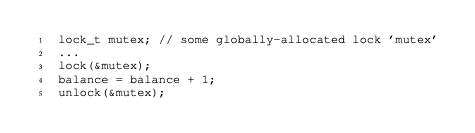
\includegraphics[width=\linewidth]{images/midterm_1_solution_1.png}
                \end{center}
                \item Is a variable with two states

                \begin{itemize}
                    \item 1 - (available/unlock/free)
                    \item 0 - (acquired/locked/held)
                \end{itemize}
            \end{itemize}

            \item \textbf{Semaphore}

            \begin{itemize}
                \item Is very easy to understand, but hard to program
                \item Is an abstract data types that provide synchronizaion
                \item Uses integer variable \texttt{count} with two atomic operations

                \begin{enumerate}[1.]
                    \item (\texttt{wait/P/decrement}) - block until \texttt{count $>$ 0} then decrement variable

                    \begin{center}
                    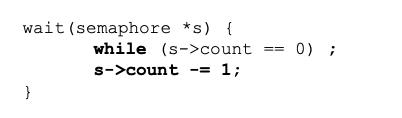
\includegraphics[width=0.8\linewidth]{images/midterm_1_solution_2.png}
                    \end{center}

                    \item (\texttt{signal/V/increment}) - increment \texttt{count}, unblock a waiting thread

                    \begin{center}
                    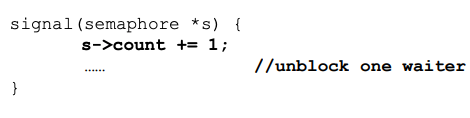
\includegraphics[width=0.8\linewidth]{images/midterm_1_solution_3.png}
                    \end{center}
                \end{enumerate}

            \end{itemize}
        \end{itemize}
    \end{enumerate}
\end{enumerate}

\end{document}